\section{Arquitectura de la solución}
\subsection{Diagrama}
La figura~\ref{fig:arq} muestra el diagrama de arquitectura (también disponible como \texttt{Diagrama\_\allowbreak Arquitectura\_\allowbreak Solucion.drawio} en la raíz del repositorio). Estado del requisito: \cumple.

\begin{figure}[htbp]
\centering
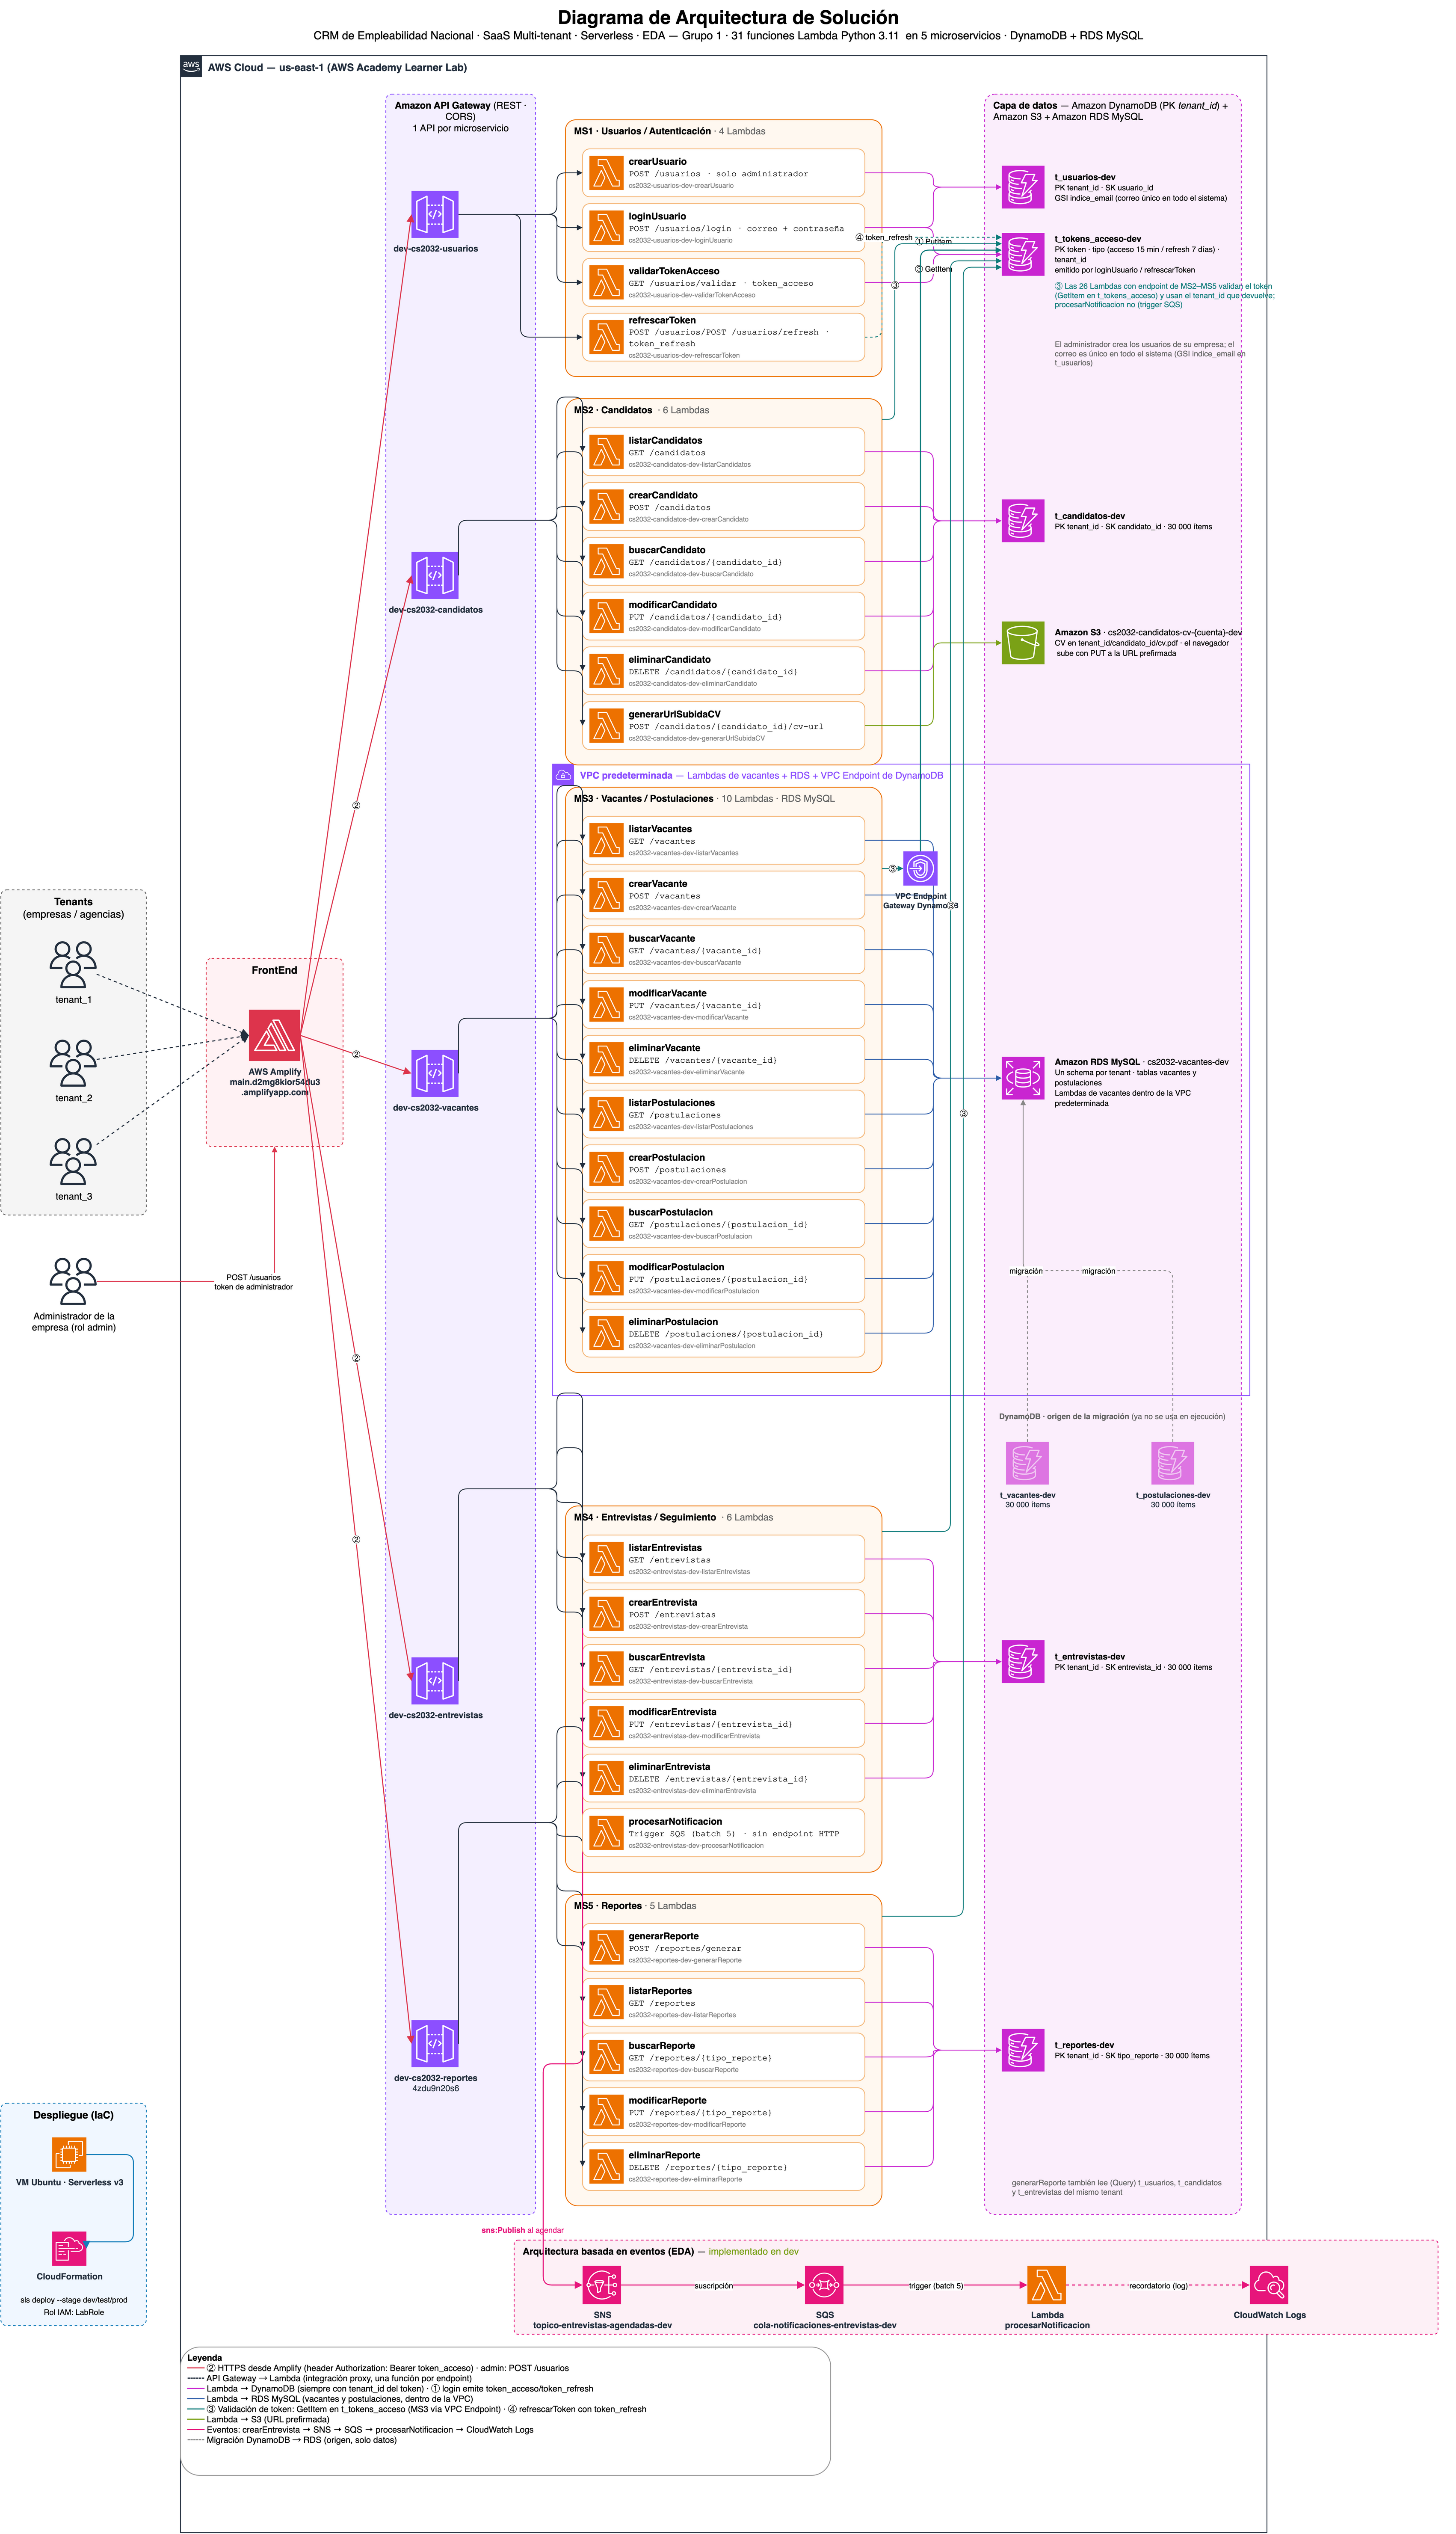
\includegraphics[height=0.82\textheight,width=\textwidth,keepaspectratio]{figuras/Diagrama_Arquitectura_Solucion.png}
\caption{Diagrama de arquitectura de la solución.}\label{fig:arq}
\end{figure}

\subsection{Explicación por capas}
\begin{longtable}{p{3cm}p{11cm}}
\toprule
\textbf{Capa} & \textbf{Componentes} \\
\midrule
\endhead
Presentación & Frontend estático (HTML, CSS, JS) en AWS Amplify, que consume las cinco APIs. \\
API & Cinco APIs REST de API Gateway (\texttt{dev-cs2032-usuarios}, \texttt{-candidatos}, \texttt{-vacantes}, \texttt{-entrevistas}, \texttt{-reportes}). \\
Cómputo & 31 funciones Lambda Python 3.11, una por endpoint, empaquetadas individualmente con un módulo \texttt{common/} compartido. \\
Autenticación & Tablas propias \texttt{t\_usuarios-dev} y \texttt{t\_tokens\_acceso-dev}; cada servicio valida el \texttt{Bearer} con \texttt{get\_item} en la tabla de tokens (no se usa Cognito). \\
Datos & DynamoDB (usuarios, tokens, candidatos, entrevistas, reportes) con \texttt{tenant\_id} como partition key; RDS MySQL 8.0 (vacantes y postulaciones) con un schema por tenant. \\
Almacenamiento & S3: bucket de CVs con URL prefirmada PUT. \\
Mensajería (EDA) & SNS \texttt{topico-entrevistas-agendadas-dev}, SQS \texttt{cola-notificaciones-entrevistas-dev}, Lambda \texttt{procesarNotificacion}. \\
Red & VPC predeterminada \texttt{vpc-0fac6f2d1ab59f1fa}; endpoints de DynamoDB (gateway) y SNS (interface); Lambdas de vacantes, \texttt{crearEntrevista} y \texttt{generarReporte} dentro de la VPC. \\
Despliegue & Serverless Framework v3; un \texttt{serverless.yml} por servicio, un stack CloudFormation por servicio. \\
\bottomrule
\end{longtable}

\subsection{Multi-tenancy}
\begin{itemize}
\item \textbf{DynamoDB:} \texttt{tenant\_id} es partition key de las tablas de negocio; su valor se toma del token validado, nunca del body ni de la URL.
\item \textbf{RDS:} patrón \emph{Single Database, Multiple Schemas}: una instancia \texttt{cs2032-vacantes-dev} (MySQL 8.0.46, db.t3.micro, Single-AZ, no pública, sin cifrado) con un schema por tenant.
\item \textbf{S3:} prefijo \texttt{tenant\_id/candidato\_id/cv.pdf}.
\end{itemize}
Estado: \cumple. La prueba de aislamiento (sección~\ref{sec:pruebas}) confirma que \texttt{tenant\_2} recibe 404 sobre recursos de \texttt{tenant\_1}.

\subsection{Evidencia de red y seguridad}
\ev{05\_vpc\_seguridad.txt}:
\begin{tabular}{@{}lll@{}}
\toprule
Recurso & Identificador & Detalle \\
\midrule
VPC & \texttt{vpc-0fac6f2d1ab59f1fa} & 172.31.0.0/16, available \\
Endpoint DynamoDB & \texttt{vpce-06ffe41b6ff20907a} & Gateway, available \\
Endpoint SNS & \texttt{vpce-0c5e6af041ebd0462} & Interface, available \\
Security group & \texttt{sg-01975563d890002a4} & Entrada solo desde el propio SG (todo y 3306); salida 0.0.0.0/0 \\
\bottomrule
\end{tabular}
